\documentclass[a4paper]{article}

\usepackage{numprint}
\usepackage{nameref}
\usepackage{float}
\usepackage{url}
\usepackage{graphicx}	% For figure environment
\usepackage{epstopdf}
\usepackage[center]{subfigure}
\usepackage{amssymb}	% For mathematical figures like \mathbb{R}
\usepackage{amsmath}
\usepackage{framed}
\usepackage{tikz}
\usetikzlibrary{mindmap,trees}
\usepackage{pdflscape}
\usepackage[a4paper]{geometry}
\usepackage{subfiles}
\usepackage{listings}
\usepackage{color}

\definecolor{dkgreen}{rgb}{0,0.6,0}
\definecolor{gray}{rgb}{0.5,0.5,0.5}
\usepackage{array}
\usepackage{booktabs}% http://ctan.org/pkg/booktabs
\usepackage{xparse}% http://ctan.org/pkg/xparse
% Rotation: \rot[<angle>][<width>]{<stuff>}
\NewDocumentCommand{\rot}{O{45} O{1em} m}{\makebox[#2][l]{\rotatebox{#1}{#3}}}%
\definecolor{mauve}{rgb}{0.58,0,0.82}

\lstset{frame=tb,
  language=Java,
  aboveskip=3mm,
  belowskip=3mm,
  showstringspaces=false,
  columns=flexible,
  basicstyle={\small\ttfamily},
  numbers=none,
  numberstyle=\tiny\color{gray},
  keywordstyle=\color{blue},
  commentstyle=\color{dkgreen},
  stringstyle=\color{mauve},
  breaklines=true,
  breakatwhitespace=true
  tabsize=3
}


\title{Advanced Systems Lab - Milestone I} 
\author{Lukas Elmer, Matthias Ganz} 
\date{\today} 


\begin{document}

\maketitle

\pagebreak

\tableofcontents

\pagebreak

\begin{abstract}

This document, describes the message queuing system which was build. Architecture and design choices are shown and explained. Further test scenarios and test loads are defined. Resulting test output is described and analysed.

\end{abstract}



%% ----------------------------------------------
% Section Messaging System
%% ----------------------------------------------
\section{Messaging System}
In this section the system under test (also named as \textbf{middle ware}  or \textbf{broker}) is described.


%% ----------------------------------------------
\subsection{Overview}

Figure \ref{fig:system-overview} shows a generic setup of the messaging system. Multiple middle ware components are connected to a single database and severs a couple of clients. Application state is persisted on the database, therefore a middle ware component can be considered as stateless.

% ------------------------------------------------
% Figure - system overview

\begin{figure}[H]
  \begin{center}
    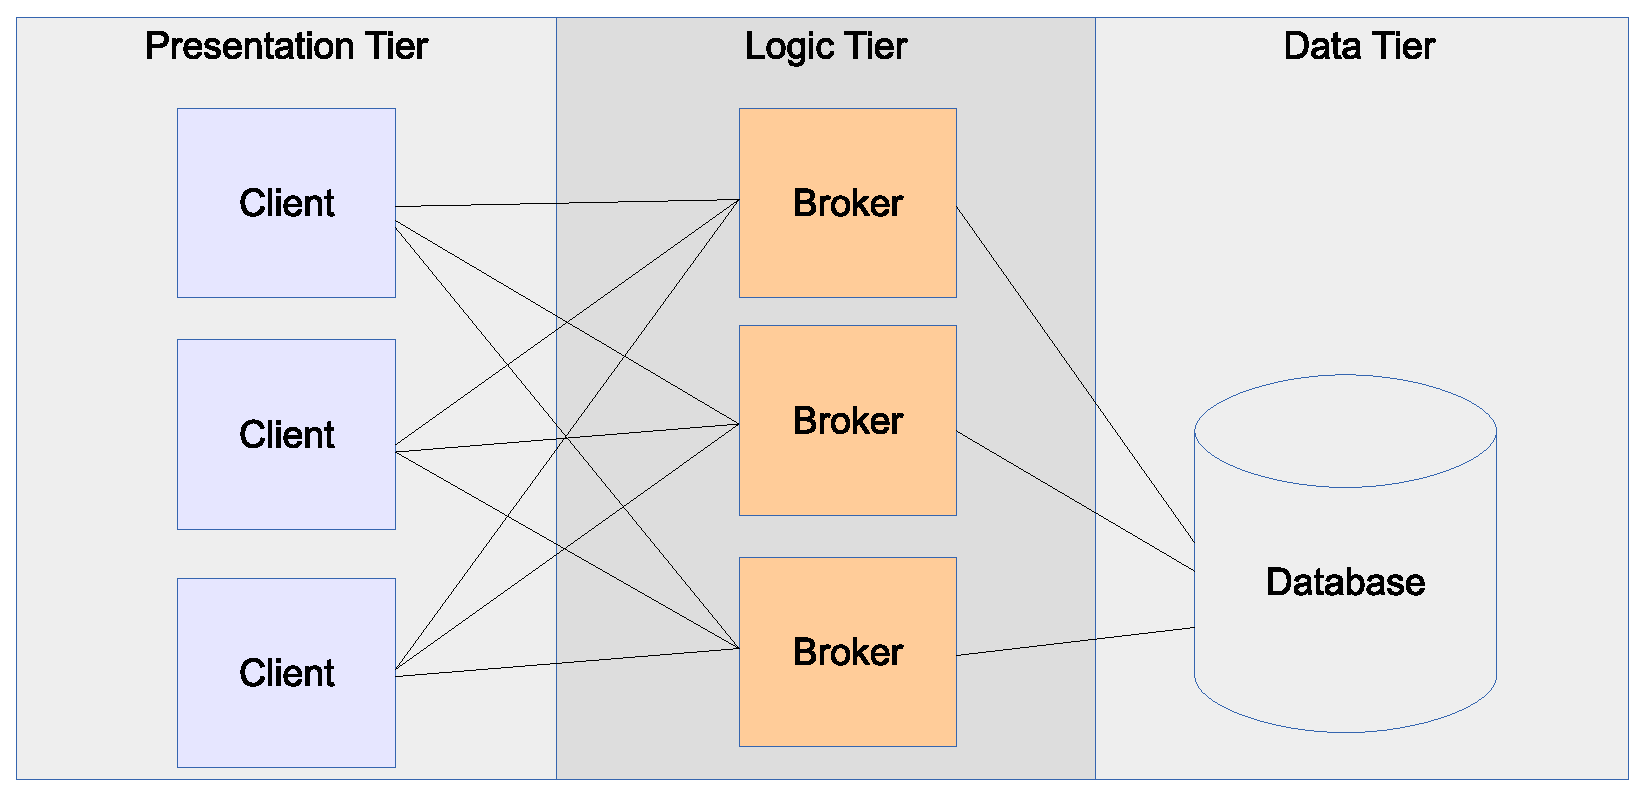
\includegraphics[scale=0.5]{../drawings/system-overview.eps}
  \end{center}
  \caption{System Overview}
  \label{fig:system-overview}
\end{figure}

Figure \ref{fig:middleware-threading} shows important software components of a single middle ware. A nonblocking network interface (NIO) handles communication to the clients. Received data is put to a single thread safe request queue.

A configurable number of workers are constantly reading from the request queue. As soon as a worker gets a piece of work (request raw data) it then performs the following tasks:
\begin{itemize}
\item decoding: The raw request is parsed and converted into a request java object
\item process: The request is processes. The database is accesses and a response object is created
\item encode: The response object is serialized and placed into the response queue of the network interface.
\end{itemize}

% ------------------------------------------------
% Figure - threading

\begin{figure}[H]
	\begin{center}
    \includegraphics[scale=0.5]{../drawings/broker-threading.eps}
  \end{center}
  \caption{Middleware's main Components}
  \label{fig:middleware-threading}
\end{figure}

%% ----------------------------------------------
\subsection{Client to Middleware Interface}

\subfile{part01-10-clientinterface.tex}

%% ----------------------------------------------
\subsection{Database Design}

TODO

%% ----------------------------------------------
\subsection{Middleware to Database Interface}

TODO


%% ----------------------------------------------
% Section Design Decisions
%% ----------------------------------------------
\subfile{part02-design.tex}


%% ----------------------------------------------
% Section Performance Relevant Features
%% ----------------------------------------------
\subfile{part03-features.tex}

%% ----------------------------------------------
% Section Experiments
%% ----------------------------------------------
\subfile{part04-experiments.tex}

%% ----------------------------------------------
% Section How to Run the system
%% ----------------------------------------------

\section{How to run the System}

This section describe all the important things laying around the core messaging system.

\subsection{Database setup}

To setup the database required for the middle ware there are two options
how to create one.

\subsubsection{Automatic setup}
You can run the java class \textit{ch.ethz.mlmq.main.Main} which is located in the main project folder \textit{mlmq}. Run the class without parameters to get usage informations.

Sample Start parameters may look like this:

\begin{verbatim} 
java ch.ethz.mlmq.main.Main dbscript -url jdbc:postgresql://localhost:5432 -db mlmq -user myusername -password mypassword -createDatabase -createTables
\end{verbatim}

\subsubsection{Manual setup}
Use your favourite database management tool (pgadmin) and execute the following sql scripts which can be found here:

\begin{verbatim} 
resource/db/001_table_create.sql
resource/db/002_stored_procedures.sql
\end{verbatim}

\subsection{Configuration}
Configurating software components is done with properties file. \footnote{See \url{http://docs.oracle.com/javase/tutorial/essential/environment/properties.html} for further information.}
\subsubsection{Main Configuration}
\label{subsub:MainConfig}

Have a look at the example configuration located at the following place.

\begin{verbatim} 
resource/config.example.properties
\end{verbatim}

Most of the configuration should be self explanatory. An exception may be the the part which is dynamically generated part when executed via test infrastructure (see figure \ref{fig:SampleConfig}). This part of the configuration describes the configuration of an experiment.

\begin{verbatim} 
common.scenario.mytype
\end{verbatim}
Describes whether this configuration file belongs to a client or a middle ware instance.

\begin{verbatim} 
common.scenario.myposition = n
\end{verbatim}
Together with \textit{common.scenario.mytype} it determines whether to pick the n-th configuration from\textit{ common.scenario.mapping.broker} or \textit{common.scenarion.mapping.client}.

\begin{verbatim} 
common.scenario.mapping.broker=...
\end{verbatim}
Lists the Broker scenarios to use. Where the first item corresponds to a class name followed by ip address and port

\begin{verbatim} 
common.scenario.mapping.client=...
\end{verbatim}
Lists the client scenarios to use. Where the first item corresponds to a class name followed by ip address.

\begin{figure}[H]
\begin{verbatim} 

...

##################################################
# Dynamically generated per test run from here on
##################################################

...

# Scenario mapping format: name1:ip,ip,ip,...;name2:ip,ip,...;name3:ip,ip,...
# E.g. scenario.mapping = broker:127.0.0.1,192.168.0.2;client:127.0.0.1,192.168.0.1
# Here: only one broker and one client
common.scenario.mapping.broker = SimpleShutdownBroker#127.0.0.1:8099;SimpleShutdownBroker#127.0.0.1:8100,127.0.0.1:8101
common.scenario.mapping.client = SimpleSendClient#127.0.0.1;SimpleSendClient#127.0.0.1;SimpleSendClient#127.0.0.1;SimpleSendClient#127.0.0.1,127.0.0.1

# either broker or client
common.scenario.mytype = client

# If the position is 5 and mytype is a broker, then this means that this is the 5th broker
# myposition starts at position 0
common.scenario.myposition = 0

...

\end{verbatim}
\caption{Sample Config}
\label{fig:SampleConfig}
\end{figure}  	

\subsubsection{Logging Configuration}
\label{subsub:loggingConfig}
Both the messaging system and the client implementation use \textit{java.util.logging.*} to log system events like errors, component startup/shutdown. This log is completely separated from the performance log (see \ref{subsub:PerfLogConfig} ), which is performed on a separate basis.

A valid logging configuration can be found here

\begin{verbatim} 
resource/logging.properties
\end{verbatim}

\subsubsection{Performance Logging Configuration}
\label{subsub:PerfLogConfig}

As already state performance logging is separated from the default logging. Any activity which may be interesting to measure is logged via this performance logger. This logger is configured via the main configuration file (see \ref{subsub:MainConfig}) and is kept simple. You just specify a path where the performance logger puts the file

\begin{verbatim} 
# folder where to write the performance log
common.performancelogger.logfilepath = performance_log
\end{verbatim}

\subsection{Start a Middleware instance/Client}
As soon as both main and logging configuration files are prepared starting the middle ware instance is easy. Just specify both files via command line arguments like the following:

\begin{verbatim} 
java ch.ethz.mlmq.main.Main scenario -config resource/brokerconfig.properties -l resource/logging.properties
\end{verbatim}

Since configuration whether to start as a client or as a server is located inside the main configuration file a client is started in the same way as a middle ware.

\subsection{Command Line Interface}

Both client and middle ware instance can be controlled using basic commands. These commands are written into the so called command file which is configured in the main configuration like this.

\begin{verbatim}
common.commandofile.path = commando.txt
\end{verbatim}

While the client or the middle ware instance is running one can write a single command into this file to be executed. The middle ware periodically checks whether the file has changed. If so it tries to execute the command contained in the file.

\begin{figure}[H]
  \begin{center}
\begin{tabular}{|c|l|}
\hline 
command & description \\ 
\hline 
shutdown & Gracefully shuts down the middleware \\ 
logstacktrace & Writes the current stack trace of all threads in the virtual machine to the log \\ 
logmemory & Writes the current memory consumption to the log \\ 
\hline
\end{tabular} 
  \end{center}
  \caption{Commando File Commands}
\end{figure}


\subsection{Logging}
This chapter describes what is logged rather than how the logging is configured. (Check \ref{subsub:PerfLogConfig} and \ref{subsub:loggingConfig} to see how the logging is configured).

As stated logging is performed with \textit{java.util.logging}. This files are for debugging purposes only.

The \textbf{PerformanceLog} contains timing data which are used to reason about the timing behaviour of the system which has been build.

Except for the first line of the file the structure of the \textbf{PerformanceLog} has a csv file format.


\subsubsection{Columns} represent the following values
\begin{enumerate}
\item Time taken for a specific action
\item UTC timestamp when a specific action was finished
\item Name of the action
\item Different runtime dependant context information. (E.g. C[.] indicates the number of connected clients on a middle ware instance)
\end{enumerate}

\subsubsection{Action Names}
\label{subsub:PerfLogger-ActionNames}
The following list shows the different types of actions which are logged and their meaning. Action names were chosen to be as short as possible to reduce log file size.

\begin{itemize}
\item \textbf{CSndReq} - request/response rountrip measured from a client's perspective 
	\begin{itemize}
	\item \textbf{BTotReqResp} - time taken from the first received byte to the last sent response byte measured from a broker's perspective.
	\item \textbf{BRcvReq} - time taken to receive a Request. This measures how long it takes to receive all request bytes on the broker.
	\item \textbf{BProcReq} - time taken by the worker. Tells you how long a single worker thread is occupied processing a certain request.
		\begin{itemize}
   		\item \textbf{BDb} - time taken to perform a specific database operation. Since this is measured by the broker jdbc network communication is included here.
   		\end{itemize}
	\item \textbf{BSndResp} - time taken to send a response.
	\end{itemize}
\end{itemize}

\subsubsection{Example Performance Log}
An example performance log is shown in figure \ref{fig:sample-perf-log}

\begin{figure}[H]
  \begin{center}
	\begin{verbatim}
BrokerConfiguration Scenario[SimpleShutdownBroker] Port[8099] WorkerThreadCount[4] DbConnectionPoolSize[4]
4;1383684920403;BRcvReq;C[9]
0;1383684920443;BRcvReq;C[10]
93;1383684920533;BDb#getClientId;C[10]
26;1383684920561;BDb#insertNewClient;C[10]
7;1383684920568;BDb#createClientQueue;C[10]
129;1383684920569;BProcReq#RegistrationRequest:RegistrationResponse;C[10]
0;1383684920570;BSndResp;C[10]
132;1383684920571;BTotReqResp;C[10]
1;1383684920571;BDb#getClientId;C[10]
14;1383684920572;BDb#createClientQueue;C[10]
166;1383684920572;BProcReq#RegistrationRequest:RegistrationResponse;C[10]
8;1383684920573;BDb#createClientQueue;C[10]
132;1383684920573;BProcReq#RegistrationRequest:RegistrationResponse;C[10]
	\end{verbatim}
  \end{center}
  \caption{Sample Performance Log}
  \label{fig:sample-perf-log}
\end{figure}

\subsection{Unit Tests}
While developing the system we strictly relied on unittests which are located in the test folder of the mlmq eclipse project.

In order to have the database related and system unittests working you may need to adjust database connection information located in the following file. This configuration file is used by all Unit Tests which need client specific configuration.

\begin{verbatim}
resource/brokerconfig.properties
\end{verbatim}

\section{Test Infrastructure}
\label{sec:TestInfrastructure}

To partially automate testing a Ruby on Rails\footnote{\url{http://rubyonrails.org}} web application was developed to help simplify running experiments on the Amazone cloud. It is refered as Testmaster.

% ------------------------------------------------
% Figure - threading

\begin{figure}[H]
	\begin{center}
    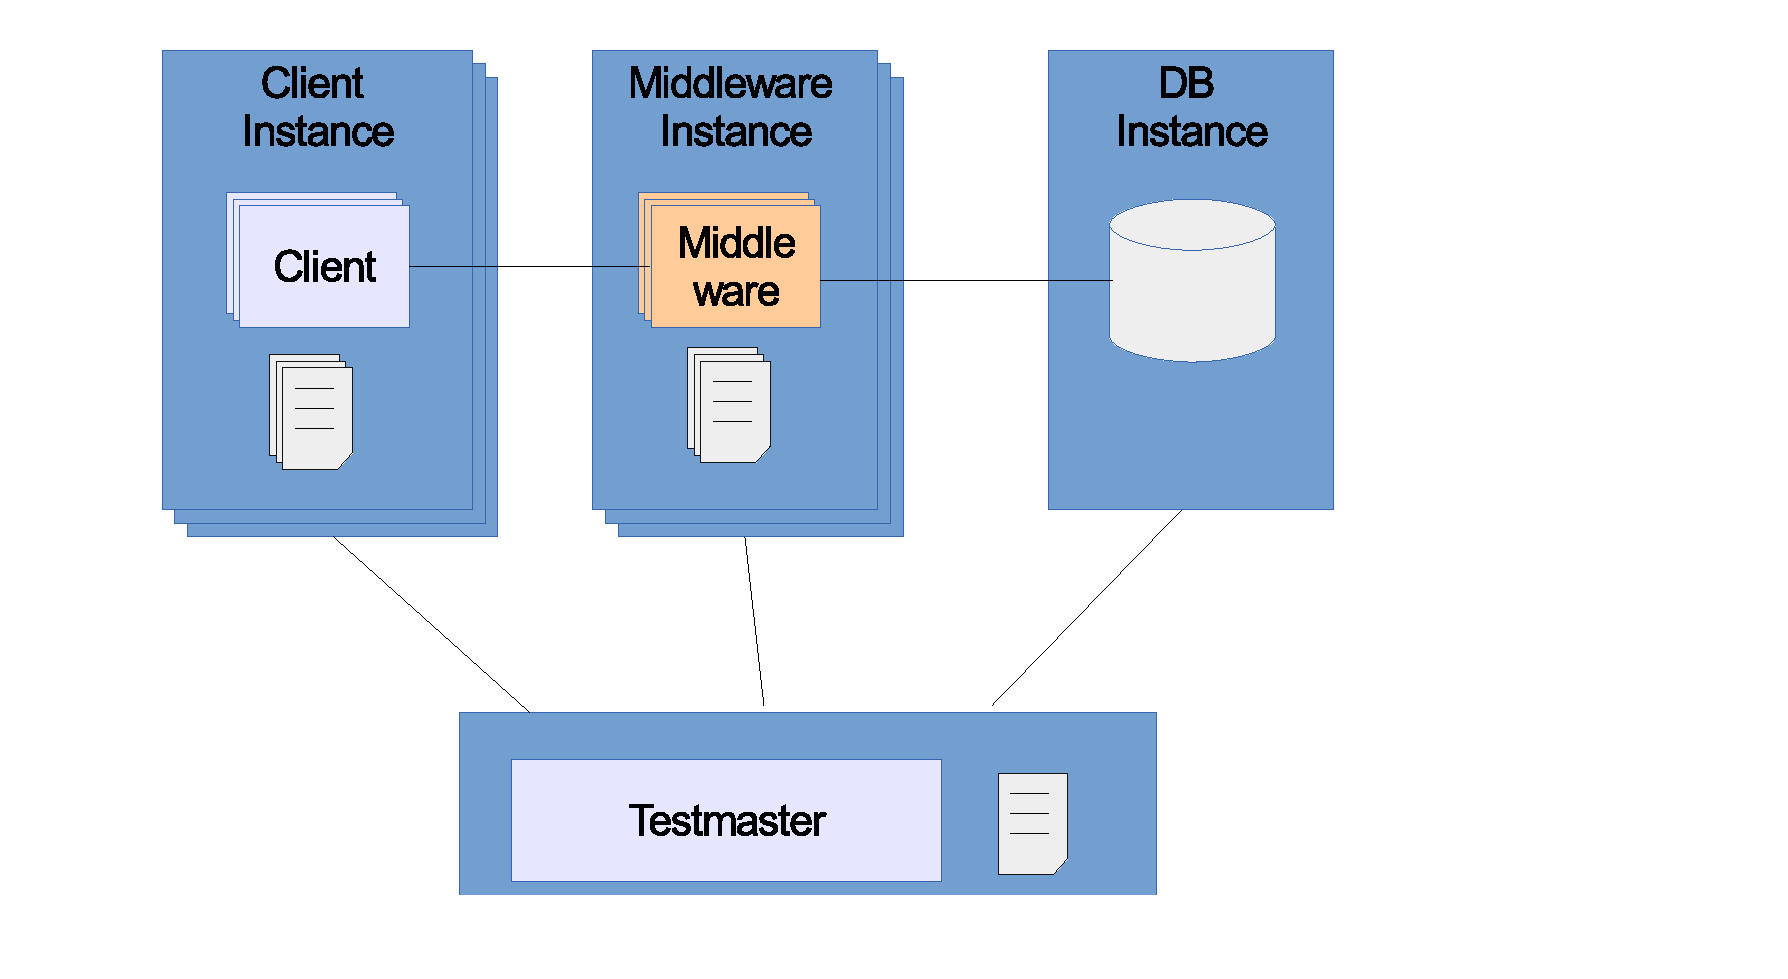
\includegraphics[scale=0.4]{../drawings/testsystem-overview.eps}
  \end{center}
  \caption{Test Master Overview}
  \label{fig:testmaster}
\end{figure}

%% ----------------------------------------------

\subsection{Workflow}

\subsubsection{Create an Experiment}
To run an experiment at first one has to define a new testrun. This is done by hand via a web interface. One has to provide the following information:

\begin{itemize}
\item Define the number middle ware instances are set up on how many Amazon instances.
\item Define the workload. This implies choosing how many instances of each client type are needed.
\item Provide client and middle ware configuration.
\end{itemize}

\subsubsection{Run an Experiment}
This step is automatically performed without user interaction. The test master performs the following steps:

\begin{enumerate}
\item Start the required Amazon instances
\item Get the latest binaries of the middleware
\item Copy the binaries and configuration to the Amazon instances
\item Start all the binaries with the required parameters
\item Periodically check whether the experiment is still running.
\item If the experiment has finished, logging information is gathered, compressed and stored on the test master
\end{enumerate}

\subsubsection{Analyze an Experiment}
As soon as an experiment has finished and all logging information is collected the web interface enables two buttons "Analyze" and "Downlodad". 

"Download" allows to get zip file with all the log files created during the experiment.

"Analyze opens a form which provides a web interface for the Log Analyzer (see \ref{subsec:LogAnalyzer}). Plots can be created with only a few clicks.

\subsection{Log Analyzer}
\label{subsec:LogAnalyzer}

In order to semi automatically analyze performance log files which have been created through the process of an experiment a Java programm was written to simplify evaluation of these files.

The project folder (See Section \ref{sec:WhereToFind:MessagingSystemSrc}) contains an Eclipse project called \textit{log\_analyzer}. All you need to do is to provide a path to the folder containing all the log files of an experiment you want to analyze. By executing the class \textit{ch.ethz.mlmq.log\_analyzer.Main} you can choose to either generate a csv file or a gnuplot file\footnote{\url{See http://www.gnuplot.info/}}.


\subsubsection{Example}
The following line of code shows an example of calling the log analyzer.

\begin{verbatim}
java ch.ethz.mlmq.log_analyzer.Main -d logs/test_run_56 -type CSndReq#OK# -fmt csv
\end{verbatim}

The folder found at logs/test\_run\_56 which contains several log files is analyzed and a csv file is created. This file contains timing information for client request/reponse operations (See \ref{subsub:PerfLogger-ActionNames}).

%% ----------------------------------------------
% Section What is where
%% ----------------------------------------------
\section{What to find where}

This section should help find code, experiment data, plots etc.

\subsection{Messaging System Source Code}
\label{sec:WhereToFind:MessagingSystemSrc}
All source code for the messaging system, clients and log analyzer can be found here.

\url{https://github.com/ganzm/AdvancedSystemsLab2013}


\subsection{Experiment Raw data}
Experiment data is located here.

\url{https://github.com/lukaselmer/ethz-asl-testmaster-data}

\subsection{Testmaster Source Code}
Ruby on Rails Testmaster source code is located here.

\url{https://github.com/lukaselmer/ethz-asl-testmaster}

\subsection{Testmaster Installation}
The Test Infrastructure as described in Section \ref{sec:TestInfrastructure}   \nameref{sec:TestInfrastructure}. This is where you find all experiment data (even the failed ones).

\url{https://testmaster-asl-eth.renuo.ch}


%% ----------------------------------------------
% Section References
%% ----------------------------------------------
\section{References}

% TODO

http://dl.acm.org/citation.cfm?id=SERIES12798.1557393

@book{hanmer2007patterns,
  title={Patterns for fault tolerant software},
  author={Hanmer, Robert},
  year={2007},
  isbn = {0470319798, 9780470319796},
  publisher={Wiley Publishing}
}

%\bibliography{mybib}

%% %%%%%%%%%%%%%%%%%%%%%%%%%%%%%%%%%%%%%%%%%%%%%%%%%%%%%%%%%%%%%%%%%%%%%%%%%
\section{Notes - to delete}

% unit test

\subsection{What should be included in this report }

\subsubsection{System Code}
\begin{itemize}
\item Code
\item Scripts for experiment
\end{itemize}

\subsubsection{Experimental data}
\begin{itemize}
\item Basic tests ans simple traces
\item Long running traces, Raw data and graphs for all experiments
\end{itemize}

\subsubsection{Written report}
\begin{itemize}
\item Architectural  diagrams
\item Interface description
\item explanation of the system design
\item Description of all experiments
\item statistical treatment of data
\item commentary analysis
\end{itemize}


\end{document}
